
% Make figure captions use the same size as the figure labels.
\captionsetup[figure]{font=small}

% ============================================================
% Denoising qualitative examples — page 1
% ============================================================

\begin{figure}[h]
\centering
\small

% \begin{tabular}{ccc}
% \textbf{Reference} &
% \textbf{Rotated (pre-denoise)} &
% \textbf{Denoised (ours)} \\[4pt]

% \includegraphics[width=0.30\linewidth]
% {supplementary_figures/difix3d_pics/eth3d_courtyard_345_0_ref.jpg} &
% \includegraphics[width=0.30\linewidth]
% {supplementary_figures/difix3d_pics/eth3d_courtyard_345_0_raw.jpg} &
% \includegraphics[width=0.30\linewidth]
% {supplementary_figures/difix3d_pics/eth3d_courtyard_345_0_denoised.jpg} \\

% \multicolumn{3}{c}
% {eth3d / courtyard / 345$^\circ$, score 4.25} \\[4pt]


% \includegraphics[width=0.30\linewidth]
% {supplementary_figures/difix3d_pics/eth3d_pipes_345_1_ref.jpg} &
% \includegraphics[width=0.30\linewidth]
% {supplementary_figures/difix3d_pics/eth3d_pipes_345_1_raw.jpg} &
% \includegraphics[width=0.30\linewidth]
% {supplementary_figures/difix3d_pics/eth3d_pipes_345_1_denoised.jpg} \\

% \multicolumn{3}{c}
% {eth3d / pipes / 345$^\circ$, score 4.25} \\[4pt]


% \includegraphics[width=0.30\linewidth]
% {supplementary_figures/difix3d_pics/eth3d_electro_330_2_ref.jpg} &
% \includegraphics[width=0.30\linewidth]
% {supplementary_figures/difix3d_pics/eth3d_electro_330_2_raw.jpg} &
% \includegraphics[width=0.30\linewidth]
% {supplementary_figures/difix3d_pics/eth3d_electro_330_2_denoised.jpg} \\

% \multicolumn{3}{c}
% {eth3d / electro / 330$^\circ$, score 4.20} \\[4pt]


% \includegraphics[width=0.30\linewidth]
% {supplementary_figures/difix3d_pics/eth3d_electro_60_3_ref.jpg} &
% \includegraphics[width=0.30\linewidth]
% {supplementary_figures/difix3d_pics/eth3d_electro_60_3_raw.jpg} &
% \includegraphics[width=0.30\linewidth]
% {supplementary_figures/difix3d_pics/eth3d_electro_60_3_denoised.jpg} \\

% \multicolumn{3}{c}
% {eth3d / electro / 60$^\circ$, score 3.80} \\[4pt]


% \includegraphics[width=0.30\linewidth]
% {supplementary_figures/difix3d_pics/eth3d_pipes_60_4_ref.jpg} &
% \includegraphics[width=0.30\linewidth]
% {supplementary_figures/difix3d_pics/eth3d_pipes_60_4_raw.jpg} &
% \includegraphics[width=0.30\linewidth]
% {supplementary_figures/difix3d_pics/eth3d_pipes_60_4_denoised.jpg} \\

% \multicolumn{3}{c}
% {eth3d / pipes / 60$^\circ$, score 3.80} \\[4pt]

% \end{tabular}
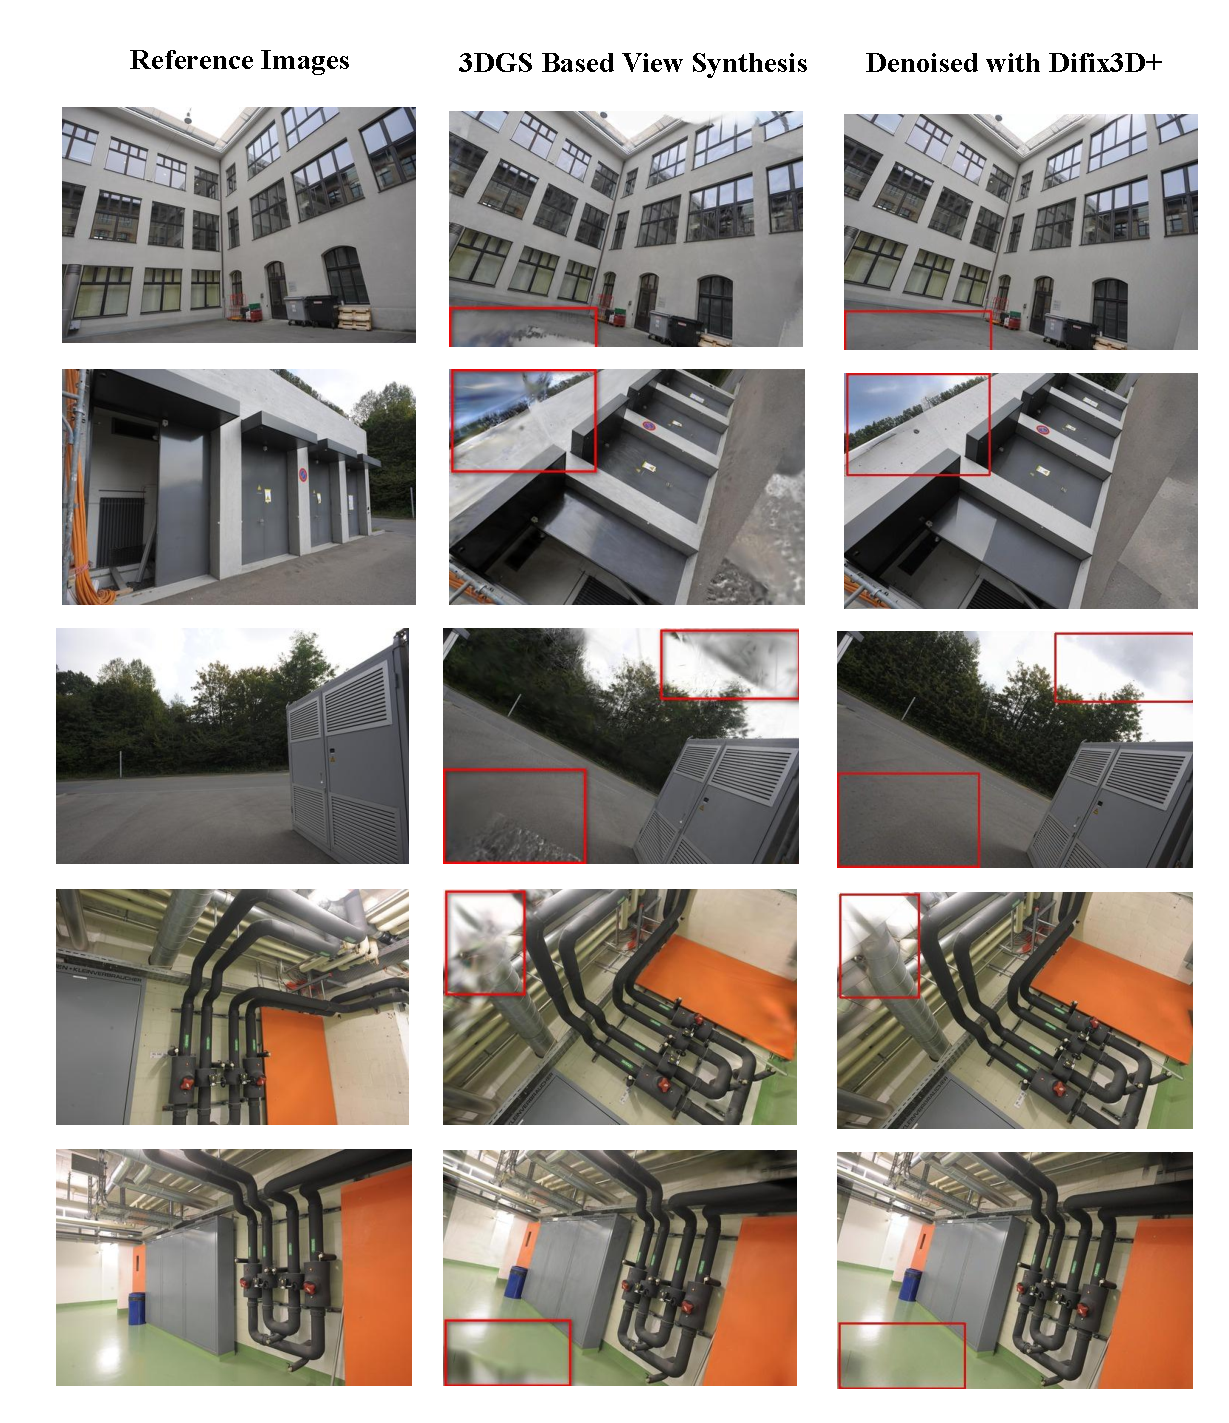
\includegraphics[width=0.98\linewidth,height=0.88\textheight,keepaspectratio]{supplementary_figures/difix3d_examples/difix-1-1.pdf}
\caption{\textbf{Effect of Difix denoising on 3DGS-based rotated view synthesis.} Reference images (left), 3DGS-synthesized views (middle), and their denoised counterparts (right), shown for the \textit{Courtyard}, \textit{Electro} and \textit{Pipes}  scenes from ETH3D. Red boxes mark artifacts in the synthesized views, with corresponding regions in the denoised views to indicate that the artifacts are removed or reduced.}
\label{fig:denoise-examples-1}

\end{figure}


% ============================================================
% Denoising qualitative examples — page 2
% ============================================================

\begin{figure}[h]
% \ContinuedFloat
\centering
\small

% \begin{tabular}{ccc}
% \textbf{Reference} &
% \textbf{Rotated (pre-denoise)} &
% \textbf{Denoised (ours)} \\[4pt]

% \includegraphics[width=0.30\linewidth]
% {supplementary_figures/difix3d_pics/tnt_Meetingroom_roll_15_5_ref.jpg} &
% \includegraphics[width=0.30\linewidth]
% {supplementary_figures/difix3d_pics/tnt_Meetingroom_roll_15_5_raw.jpg} &
% \includegraphics[width=0.30\linewidth]
% {supplementary_figures/difix3d_pics/tnt_Meetingroom_roll_15_5_denoised.jpg} \\

% \multicolumn{3}{c}
% {tnt / Meetingroom / roll 15$^\circ$, score 4.20} \\[4pt]


% \includegraphics[width=0.30\linewidth]
% {supplementary_figures/difix3d_pics/tnt_Meetingroom_roll_15_6_ref.jpg} &
% \includegraphics[width=0.30\linewidth]
% {supplementary_figures/difix3d_pics/tnt_Meetingroom_roll_15_6_raw.jpg} &
% \includegraphics[width=0.30\linewidth]
% {supplementary_figures/difix3d_pics/tnt_Meetingroom_roll_),15_6_denoised.jpg} \\

% \multicolumn{3}{c}
% {tnt / Meetingroom / roll 15$^\circ$, score 4.20} \\[4pt]


% \includegraphics[width=0.30\linewidth]
% {supplementary_figures/difix3d_pics/tnt_Church_roll_15_7_ref.jpg} &
% \includegraphics[width=0.30\linewidth]
% {supplementary_figures/difix3d_pics/tnt_Church_roll_15_7_raw.jpg} &
% \includegraphics[width=0.30\linewidth]
% {supplementary_figures/difix3d_pics/tnt_Church_roll_15_7_denoised.jpg} \\

% \multicolumn{3}{c}
% {tnt / Church / roll 15$^\circ$, score 4.00} \\[4pt]


% \includegraphics[width=0.30\linewidth]
% {supplementary_figures/difix3d_pics/tnt_Church_roll_15_8_ref.jpg} &
% \includegraphics[width=0.30\linewidth]
% {supplementary_figures/difix3d_pics/tnt_Church_roll_15_8_raw.jpg} &
% \includegraphics[width=0.30\linewidth]
% {supplementary_figures/difix3d_pics/tnt_Church_roll_15_8_denoised.jpg} \\

% \multicolumn{3}{c}
% {tnt / Church / roll 15$^\circ$, score 4.00} \\[4pt]

% \end{tabular}
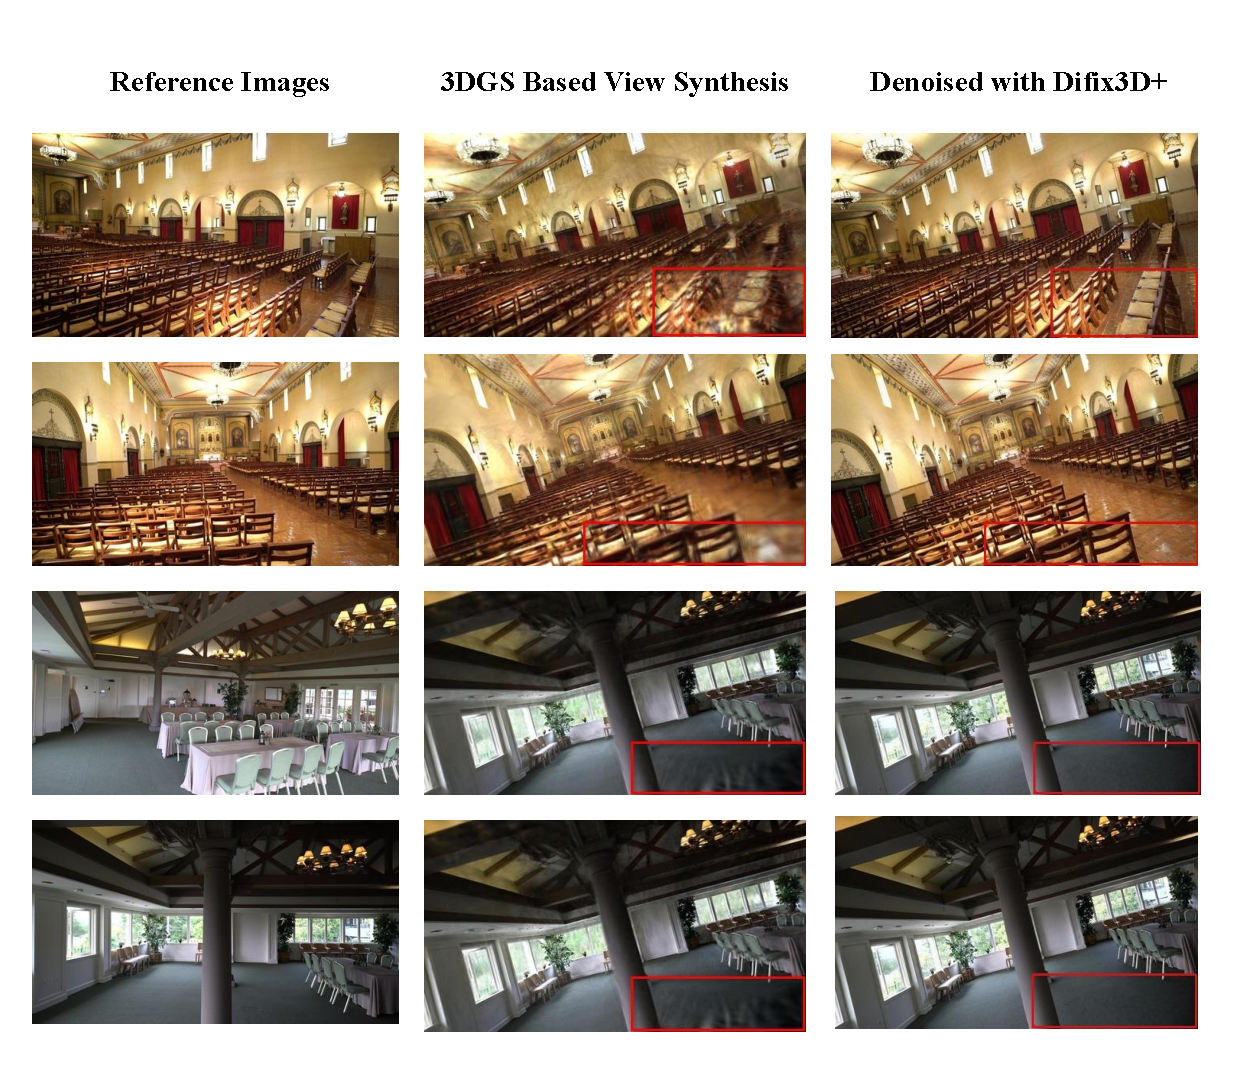
\includegraphics[width=0.98\linewidth,height=0.88\textheight,keepaspectratio]{supplementary_figures/difix3d_examples/difix-2-1.pdf}
\caption{\textbf{Effect of Difix3D denoising on 3DGS-based rotated view synthesis.} Reference images (left), 3DGS-synthesized views (middle), and their denoised counterparts (right), shown for the \textit{Church} and \textit{Meetingroom} scenes from Tanks and Temples. Red boxes mark artifacts in the synthesized views, with corresponding regions in the denoised views to indicate that the artifacts are removed or reduced.}
\label{fig:denoise-examples-2}

\end{figure}
